\chapter*{Base Station Hardware}
\addcontentsline{toc}{chapter}{Base Station Hardware}

The base station is essentially based on a main controller board and a dual power module unit shown in previous chapters. We will use the PICO controller version and the dual H-Bridge building block. Add the RailCom detectors and stir the whole soup for a while. The extension connector of the base station would still export the I2C interface and the DCC signal produced by the base station. So, adding an I2C based extension board for display, switches, etc. is of course still possible. Here is the schematic for the base station. The individual building blocks should be familiar by now. The first page shows the main controller parts. Note that it needs fewer level shifters, as most of the signals are consumed internal to the board.

\begin{figure}[htbp]
    \centering
    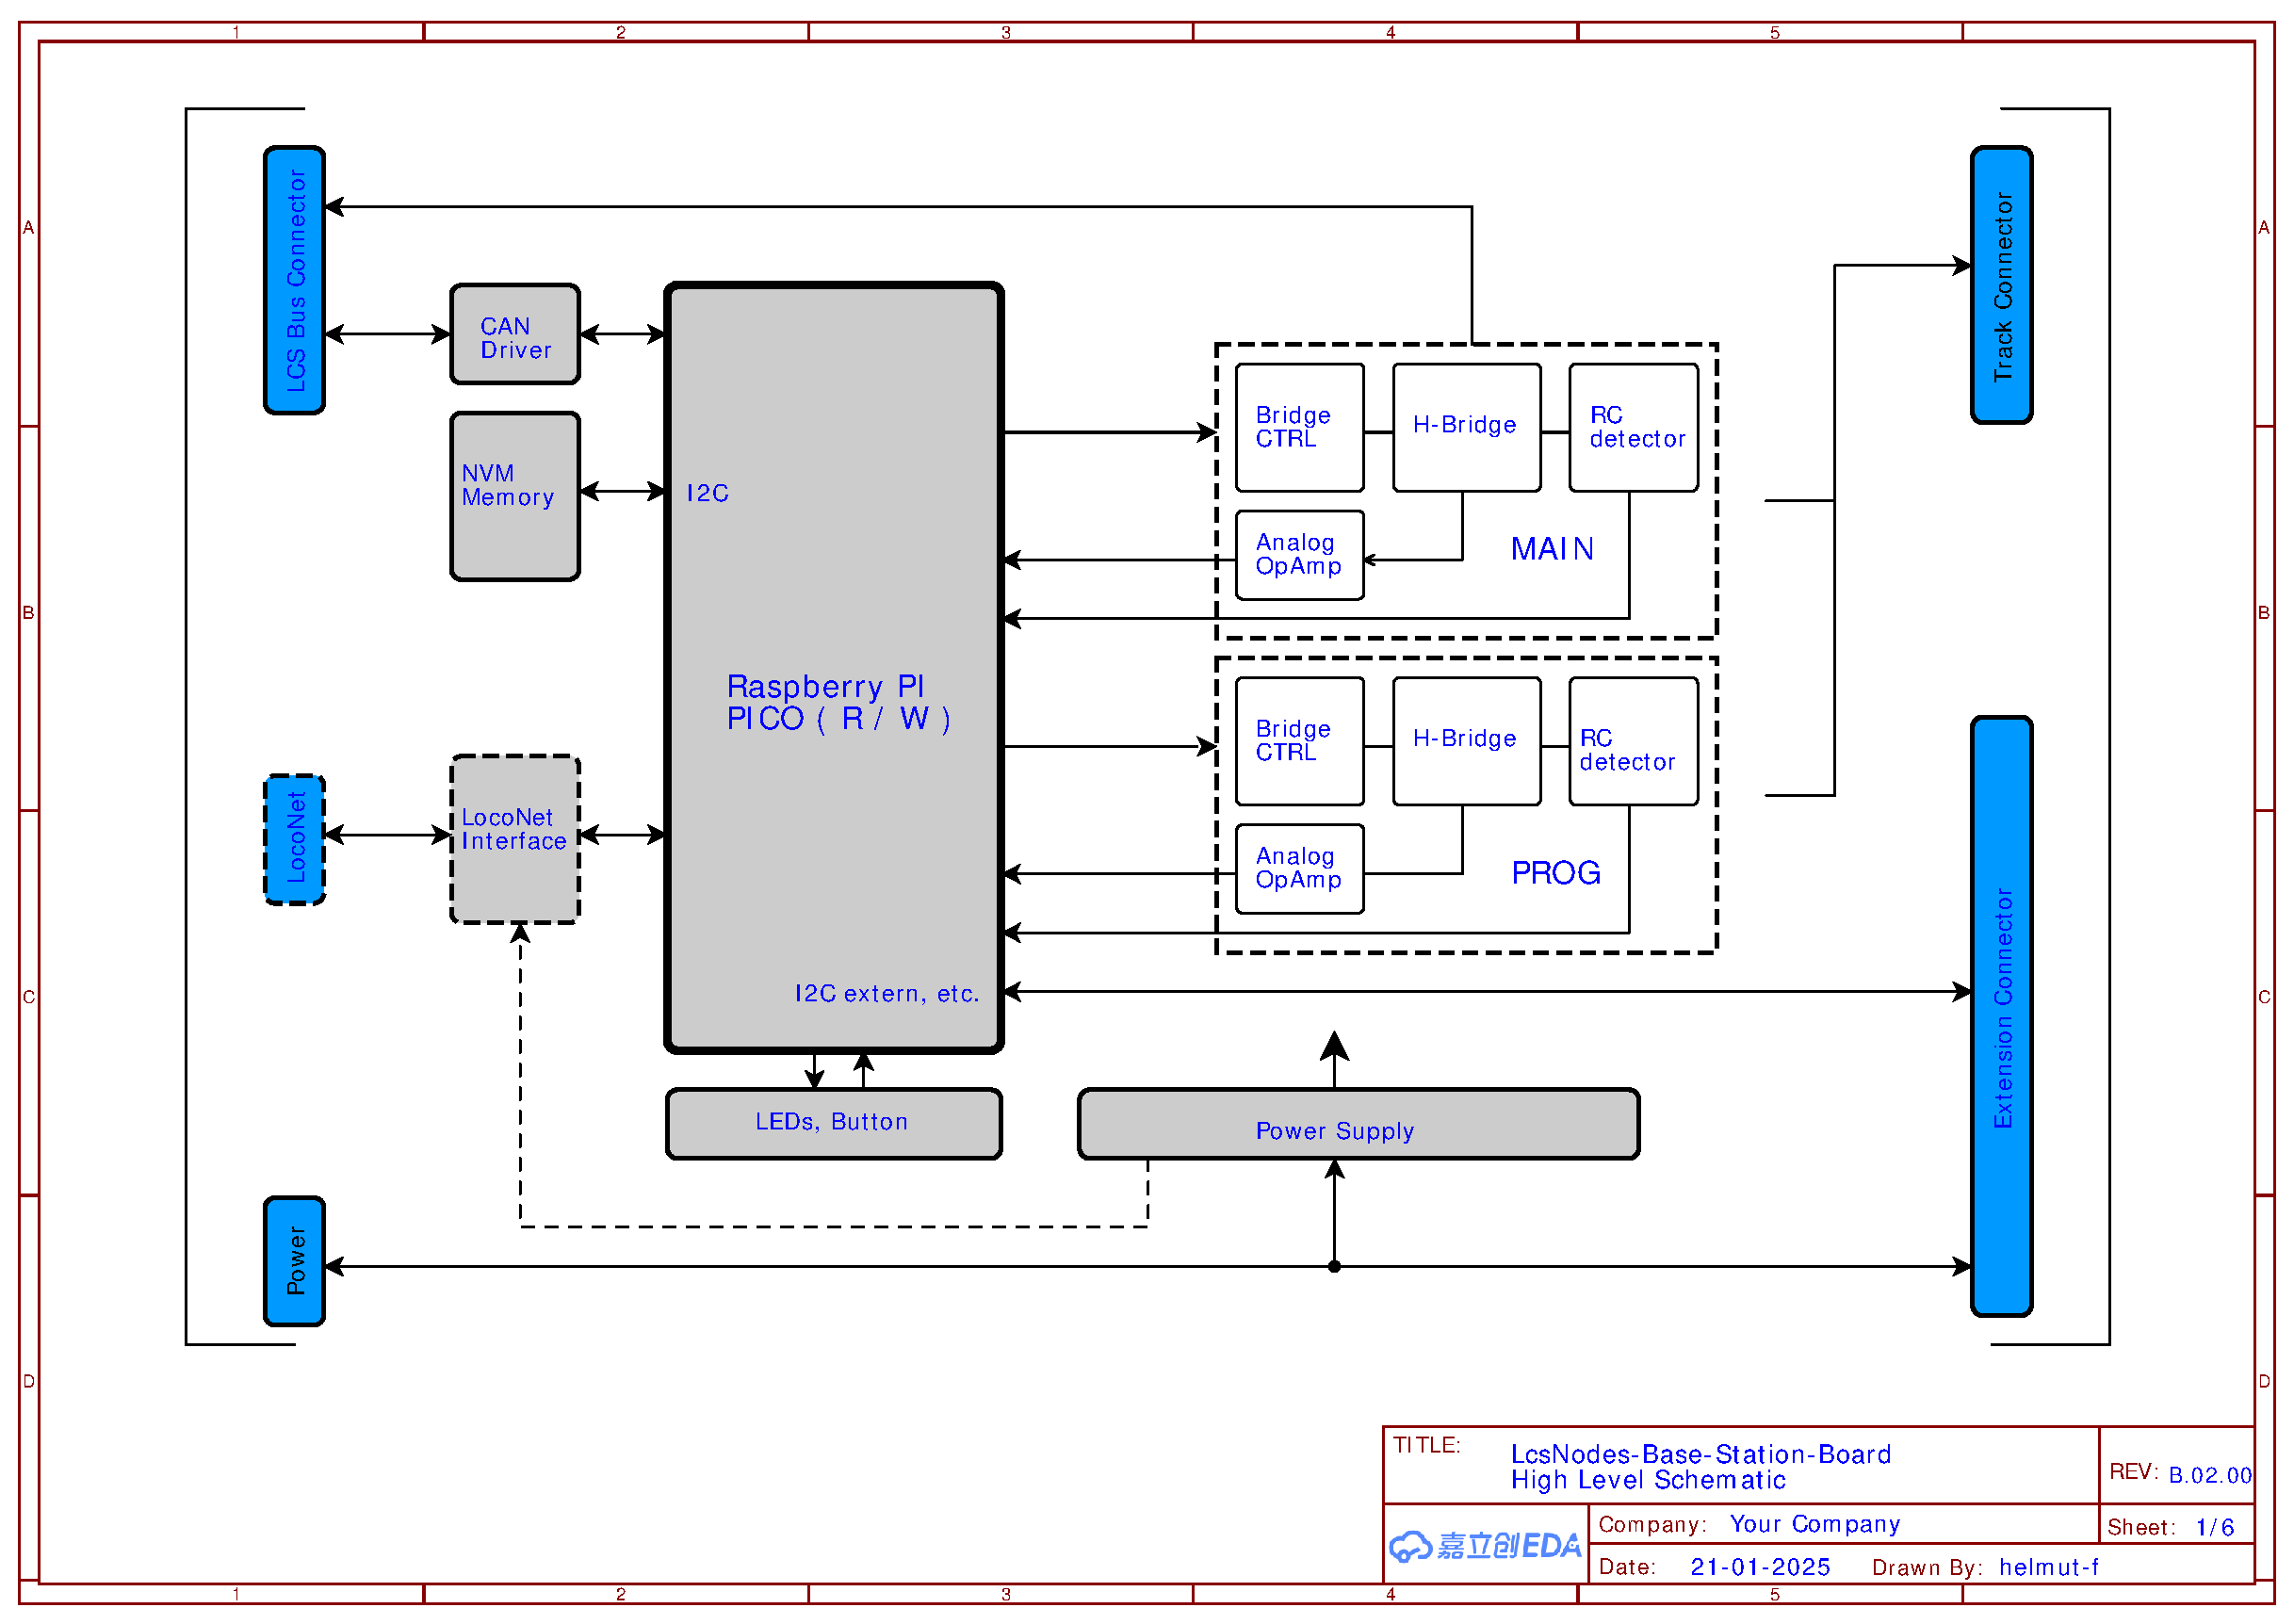
\includegraphics[page=1, width=0.9\textwidth]{schematics/Schematic_LcsNodes-Base-Station-Board.pdf}
    \caption{Base Station Block Diagram}
    %\label{fig:BlockDiagram}
\end{figure}
%\FloatBarrier

\section*{Base Station Main Controller}
\addcontentsline{toc}{section}{Base Station Main Controller}

The Raspberry PI Pico has enough capacity to implement the CAN bus protocol directly using one of the cores. As a result, only the line driver is necessary to implement the CAN bus interface. There are the level shifters for the I2C bus and a few other external signals. The Power supply needs to have a method to detect that there is an USB cable connected to the PICO and ensure that there is no conflict between the power sources. Like any LCS node, the controller needs a non-volatile memory. The base station hosts an I2C type NVM with up to 64Kbytes. The key reason for such a high capacity is that a base station might store a lot of data for each engine that it can manage.

\begin{figure}[htbp]
    \centering
    \includegraphics[page=2, width=0.9\textwidth]{schematics/Schematic_LcsNodes-Base-Station-Board.pdf}
    \caption{Base Station Main Controller}
    %\label{fig:Schematic}
\end{figure}
% \FloatBarrier

\section*{Power Module}
\addcontentsline{toc}{section}{Power Module}

The next part shows the power module. The power module exports the DCC signals via the external track power connectors and also as part of the LCS message bus connector. The track power extension connector is used by extension boards that directly use the H-Bridge output. A good example is an occupancy detector board which takes the DCC outputs and routes them to different sections, each equipped with a detectors for power consumption on the track. The power module unit features two identical channels. They are labelled "MAIN" and "PROG". Although the "PROG" channel would not need to deliver a high amperage, the dual H-Bridge is there anyway. And as said before, it would be nice to dynamically treat the PROG track as a type MAIN track too. 

\begin{figure}[htbp]
    \centering
    \includegraphics[page=3, width=0.8\textwidth]{schematics/Schematic_LcsNodes-Base-Station-Board.pdf}
    \caption{Power Module}
    %\label{fig:Schematic}
\end{figure}
\FloatBarrier

\section*{RailCom Detector}
\addcontentsline{toc}{section}{RailCom Detector}

Both channels also feature a RailCom detector. Refer to the base station firmware chapter on what we actually do with a RailCom detector. 

\begin{figure}[htbp]
    \centering
    \includegraphics[page=4, width=0.8\textwidth]{schematics/Schematic_LcsNodes-Base-Station-Board.pdf}
    \caption{RailCom Detector}
    %\label{fig:Schematic}
\end{figure}
\FloatBarrier

\section*{LocoNet Interface}
\addcontentsline{toc}{section}{LocoNet Interface}


The base station will also offer an optional LocoNet interface. One day. LocoNet is very popular communication network for model railroads and there are a lot of devices such as Cab Handhelds that connect to the LocNet bus. Wouldn't it be nice to just connect these handhelds and alike via the LocoNet bus such that they can be used as well ? I guess it would. Right now, this is work in progress, but let's already reserve the space on the board. Here is a first sketch of the interface.

\begin{figure}[htbp]
    \centering
    \includegraphics[page=5, width=0.8\textwidth]{schematics/Schematic_LcsNodes-Base-Station-Board.pdf}
    \caption{LocoNet Interface}
    %\label{fig:schematic}
\end{figure}
\FloatBarrier

\section*{ Connectors and Power}
\addcontentsline{toc}{section}{Connectors and Power}

Finally, there are the connectors and the power supplies. While the LCS node runs with 5V as before, the LocoNet interface will offer 12V on its bus to connected devices. This part is also optional if LocNot is not implemented. In addition to the basic connectors that we have as part of the LCS node design, there are also two power connectors for the two tracks.

\begin{figure}[htbp]
    \centering
    \includegraphics[page=6, width=0.8\textwidth]{schematics/Schematic_LcsNodes-Base-Station-Board.pdf}
    \caption{Connectors and Power}
    %\label{fig:schematic}
\end{figure}
\FloatBarrier

\section*{Base Station PCB}
\addcontentsline{toc}{section}{Base Station PCB}

The following picture shows the PCB for the monolithic base station. It is a 12cm by 10cm board, with the standard connectors in the usual place. As said, the LocoNet Interface is optional. 

\begin{tikzpicture}[scale=0.7, transform shape]
    \draw[help lines, gray!50, dashed] (0,0) grid( 16,8);
    \node at (8,4) {picture};
\end{tikzpicture}

Like the main controller, the monolithic base station board makes extensive use of SMD parts. While the previous boards have already been using passive SMD parts such as capacitors and resistors, this board also makes use of SMD ICs. The exception is of course the Raspberry PI PICO board and the Dual H-Bridge IC L6205. The H-Bridge is a high power part and in case of a hardware problem it can easily be replaced as a DIP version.











\section{Summary}

The base station, no matter how it is implemented, is a key component in any digital layout. It is primarily responsible for the locomotive session management and track signal generation. There could be designs where the base station is a device in a nice housing with a display, switches and so on. Other designs just put the LCS node somewhere on the layout. All these options will work just fine. And just like any other LCS node, the base station firmware offers through node and port attributes status and control functions.

The base station was also the first major LCS node with a considerable amount of hardware and software and thus went to several iterations and a considerable amount of learning curves. The very first version started with an Arduino Mega and Motor driver breakout board. The software was the original DCC++ software. The next versions actually were just a refactoring effort and work on the software. I learned a great deal on how all this works. The next base station version was a single board with all possible interfaces on an experimental PCB. It already featured CAN BUS, dual H-Bridges, and a controller, the Atmega 1284. This board served a long time for software development and further experiments. The next version of the base station was built with a main controller PCB described in the earlier chapters and a dual power unit, that also featured the RailCom detector. And again further software refactoring, refinement and learning. Finally, after a switch to the Raspberry Pi Pico controller, first on breadboard  then on PCBs, the base station shown in this chapter is the current version. The lessons learned proved to be very valuable for the overall concept development and hardware design. And in addition, there was a great deal of reading on chip specifications and, very importantly, the DCC standards. The appendix contains a list of material and web links. I highly recommend to read the electrical and DCC related standards published by the RailCommunity organization.


// ??? \textbf{note} wrap it up ..

Just like any other LCS node, the base station firmware offers through node and port attributes status and control functions. However, there is only one on the layout.

The base station was also the first major LCS node with a considerable amount of hardware and software. Initial work started with the main controller and power module extension board based on the Atmega processor family. From there, a monolithic version using the Raspberry PI PICO was developed and that is the latest base station offering.

What is next ?. Well, we have a base station and with the simple command interface it is possible to open a loco session and control that engine. But this command interface is rather for software development and debugging. What we really want is of course a handheld of some form with buttons and levers. So, before building boosters, block controller and extension boards and firmware, the next chapters will develop a handheld. 

